\documentclass{beamer}
%\usepackage[all,arc,curve,frame,color]{xy}
%\usepackage{tikz}
%\usepackage{tkz-graph}
\usepackage{mathtools}
\usepackage{ragged2e,etoolbox}
\usepackage{ulem}
\usepackage{graphicx}

\graphicspath{ {images/} }
\usepackage{amsmath,amssymb}


\newenvironment{nstabbing}
  {\setlength{\topsep}{0pt}%
   \setlength{\partopsep}{0pt}%
   \tabbing}
  {\endtabbing}

\def\jump{ \quad \\ \vspace{0.7cm} \pause}
\newcommand{\nc}{\newcommand}
\nc{\pid}{\mathfrak{p} }
\nc{\dpid}{\delta_{\mathfrak{p}}}

\def\AA{{\mathbb A}}
\def\CC{{\mathbb C}}
\def\EE{{\mathcal E}}
\def\FF{{\mathcal F}}
\def\GG{{\mathcal G}}
\def\HH{{\mathcal H}}
\def\MM{{\mathcal M}}
\def\NN{{\mathbb N}}
\def\PP{{\mathbb P}}
\def\QQ{{\mathbb Q}}
\def\RR{{\mathbb R}}
\def\ZZ{{\mathbb Z}}
\def\aa{{\mathbf a}}
\def\bb{{\mathbf b}}
\def\del{\partial}
\def\kk{\Bbbk}
\def\mm{{\mathfrak m}}
\def\nn{{\mathfrak n}}
\def\pp{{\mathfrak p}}
\def\qq{{\mathfrak q}}
\def\rr{{\mathbf r}}
\def\uu{{\mathbf u}}
\def\vv{{\mathbf v}}
\def\ww{{\mathbf w}}
\def\xx{{\mathbf x}}
\def\yy{{\mathbf y}}
\def\zz{{\mathbf z}}
\newcommand{\PGL}{\textrm{PGL}}
\newcommand{\res}{\textrm{Res}}


\DeclareMathOperator{\Tail}{Tail}
\DeclareMathOperator{\Per}{Per}
\DeclareMathOperator{\PrePer}{PrePer}
\DeclareMathOperator{\HTail}{HTail}
\DeclareMathOperator{\HPer}{HPer}
\DeclareMathOperator{\HPrePer}{HPrePer}

\makeatletter
\def\th@mystyle{%
    \normalfont % body font
    \setbeamercolor{block title example}{bg=orange,fg=white}
    \setbeamercolor{block body example}{bg=orange!20,fg=black}
    \def\inserttheoremblockenv{exampleblock}
  }
\makeatother

\makeatletter
\def\th@thmstyle{%
    \normalfont % body font
    \setbeamercolor{block title example}{bg=blue,fg=white}
    \setbeamercolor{block body example}{bg=blue!20,fg=black}
    \def\inserttheoremblockenv{exampleblock}
  }
\makeatother

\definecolor{darkgreen}{RGB}{77,153,0}
\makeatletter
\def\th@qstnstyle{%
    \normalfont % body font
    \setbeamercolor{block title example}{bg=darkgreen,fg=white}
    \setbeamercolor{block body example}{bg=green!20,fg=black}
    \def\inserttheoremblockenv{exampleblock}
  }
\makeatother

\theoremstyle{thmstyle}
\newtheorem*{mydef}{Definition}

\theoremstyle{thmstyle}
\newtheorem*{mythm}{Theorem}

\theoremstyle{thmstyle}
\newtheorem*{mynot}{Notation}

\theoremstyle{mystyle}
\newtheorem*{remark}{Remark}
\newtheorem*{conjecture}{Conjecture}
\newtheorem*{mycor}{Corollary}
\newtheorem*{mylemma}{Lemma}

\theoremstyle{qstnstyle}
\newtheorem*{question}{Question}

\usepackage{remreset}% tiny package containing just the \@removefromreset command
\makeatletter
\@removefromreset{subsection}{section}
\makeatother
\setcounter{subsection}{1}

\newcommand\Wider[2][3em]{%
\makebox[\linewidth][c]{%
  \begin{minipage}{\dimexpr\textwidth+#1\relax}
  \raggedright#2
  \end{minipage}%
  }%
}

\mode<presentation>{\usetheme{CambridgeUS}\usecolortheme{dolphin}} 
%\setbeamertemplate{navigation symbols}{}
\setbeamertemplate{blocks}[rounded][shadow=false]


\title[Primos guassianos]{Numeros Primos\\ en los\\ Enteros Gaussianos}
\subtitle[Dissertation Defense]{Dissertation Defense}
\author[Sebastian Troncoso]{Sebastian Troncoso}
\institute[BSC]{Birmingham-Southern College}
%\titlegraphic{\includegraphics[height=1.5cm]{../images/normale_pisa.png}}
\date[28 de Marzo]{ 28 de Marzo del 220. \\ \vspace{1cm} }


%\AtBeginSection[]{} % for optional outline or other recurrent slide
\AtBeginSection{\frame{\sectionpage}}
\begin{document}

\begin{frame}
\titlepage
\end{frame}

\begin{frame}
\frametitle{Resumen:}

\begin{enumerate}
\item PARTE I: Sistemas de Numericos
\begin{itemize}
\item $\NN$
\item $\QQ$
\item $\RR$
\item $\CC$
\end{itemize}

\pause
\item PARTE II: Numeros Gaussianos
\begin{itemize}
\item Operaciones $+$ y $*$
\item Primos Gaussianos
\end{itemize}

\pause
\item PARTE III: 
\begin{itemize}
\item Sobre mi

\item Preguntas
\end{itemize}
\end{enumerate}
\end{frame}

\begin{frame}
\frametitle{Los Numeros Naturales:}
\begin{center}
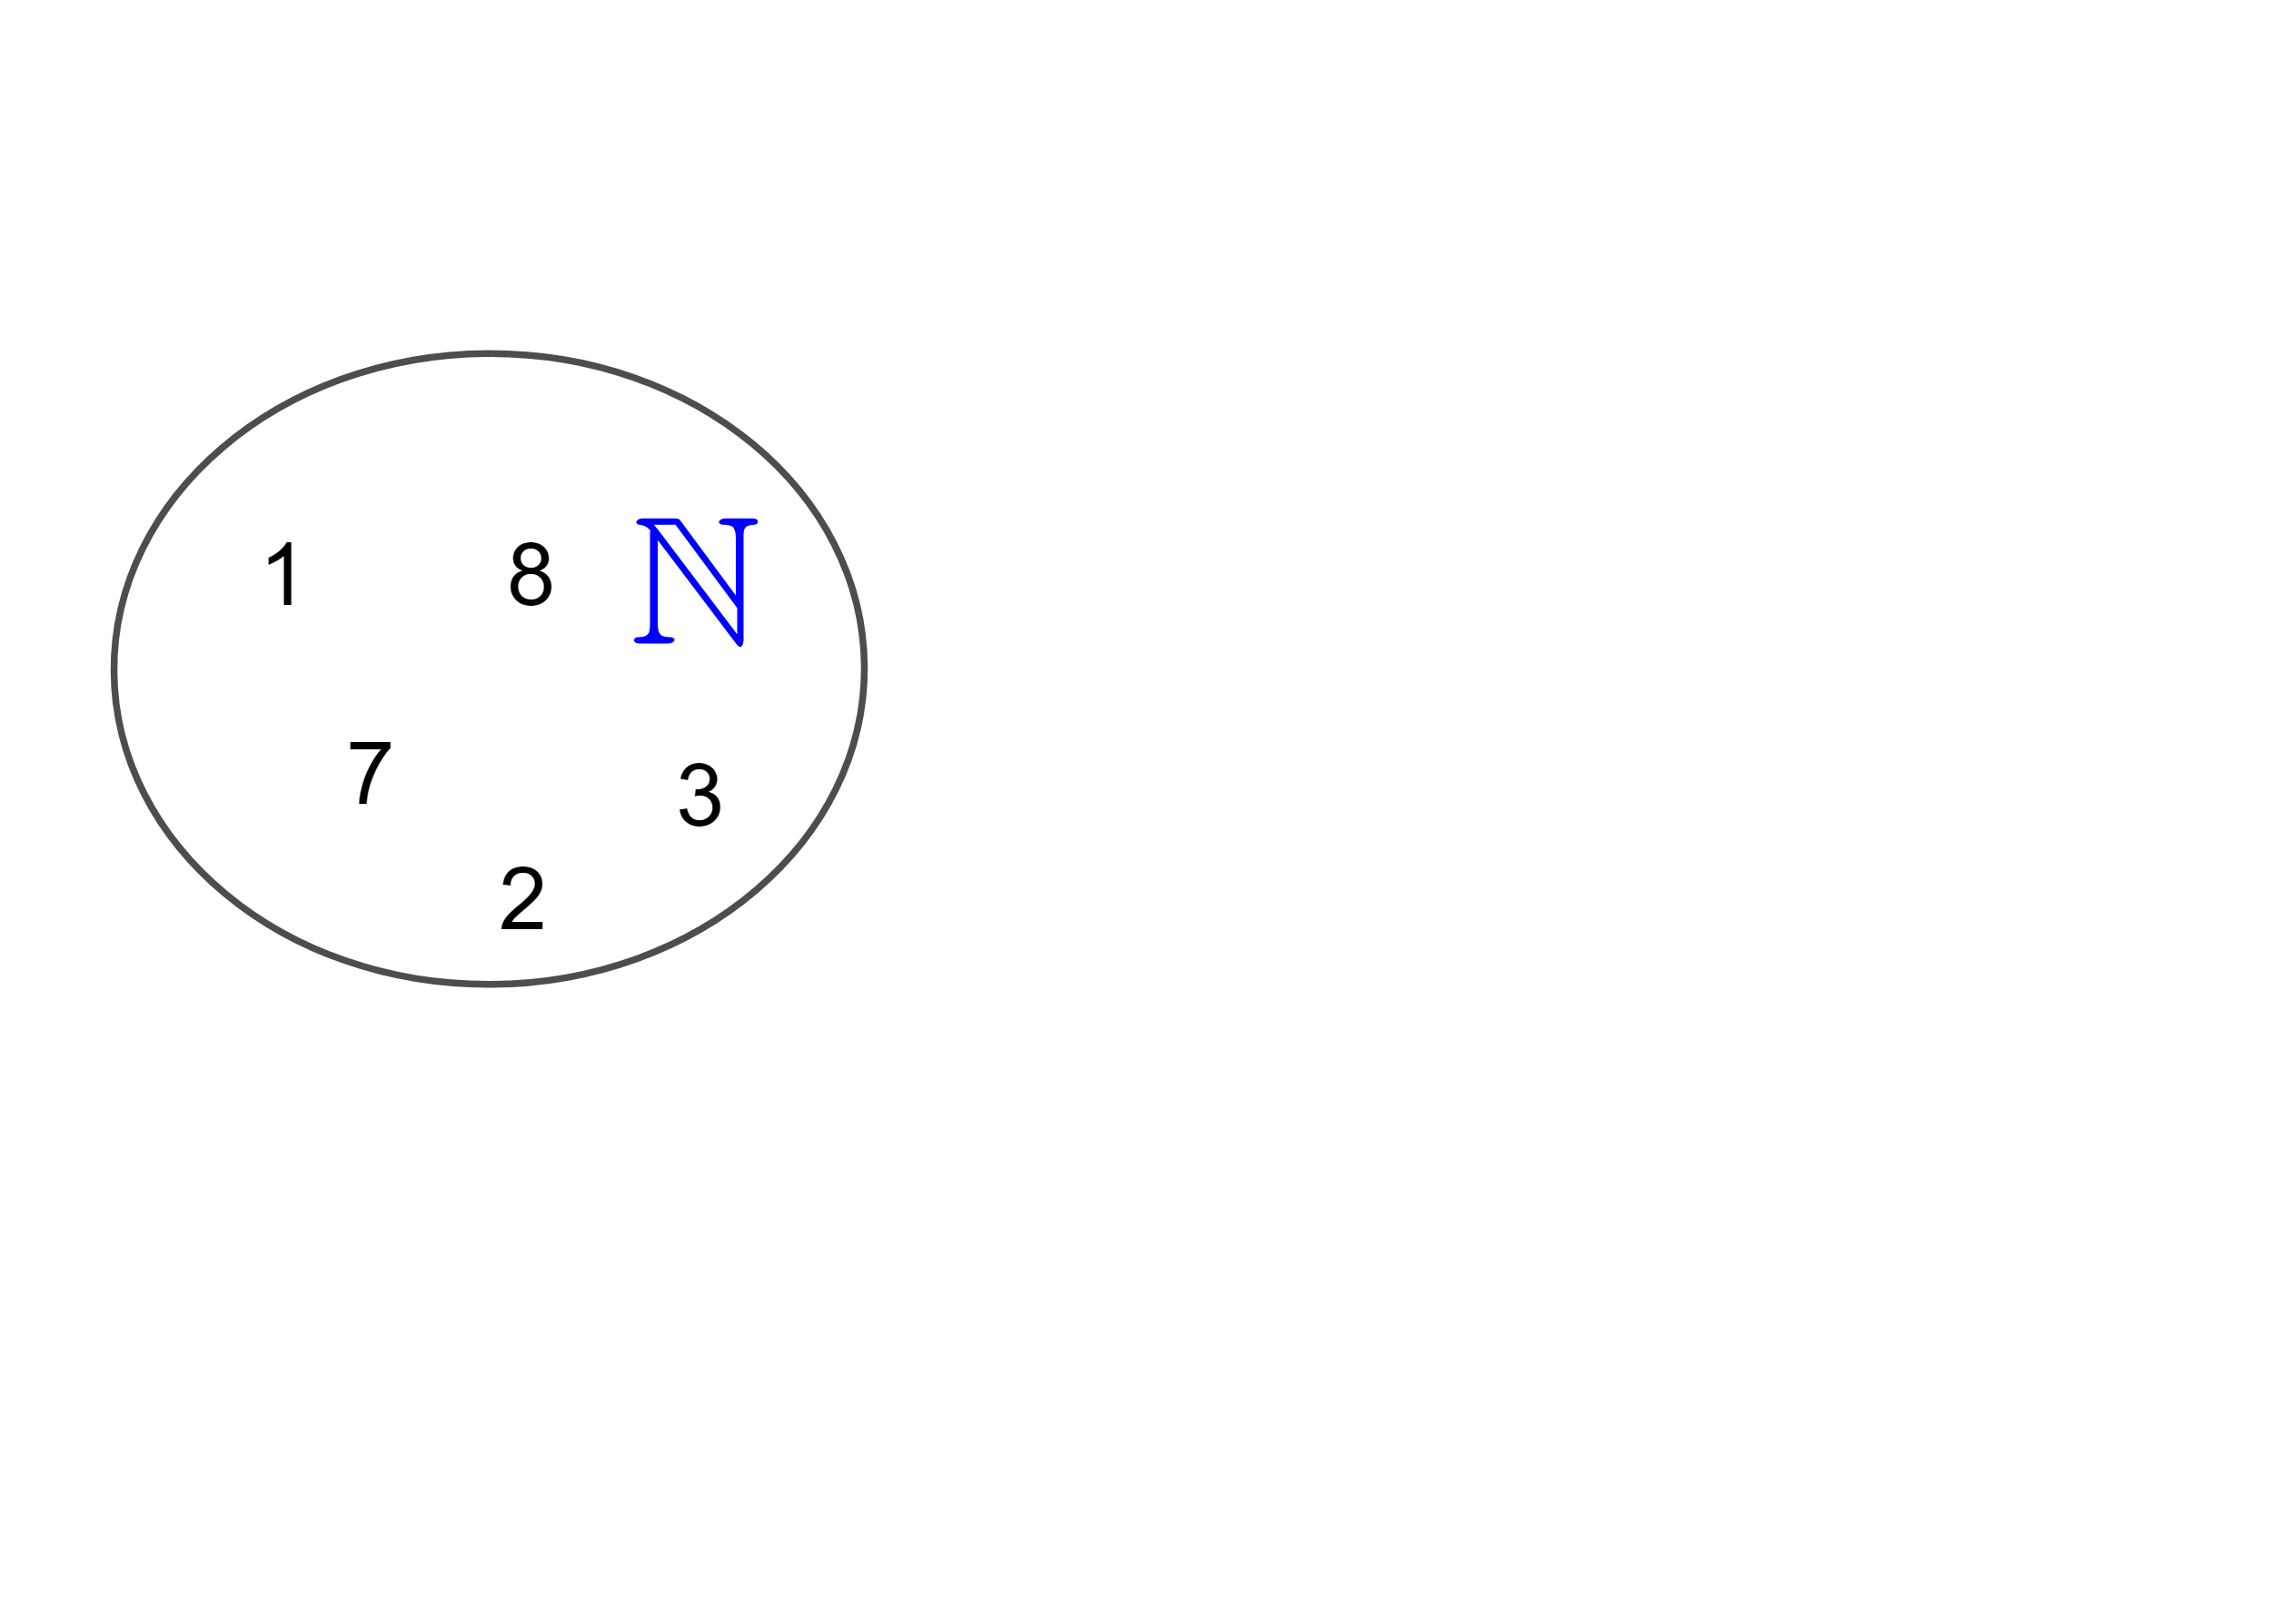
\includegraphics[width=\linewidth]{Image1.png}
\end{center}
\end{frame}

\begin{frame}
\frametitle{Los Numeros Cardinales:}
\begin{center}
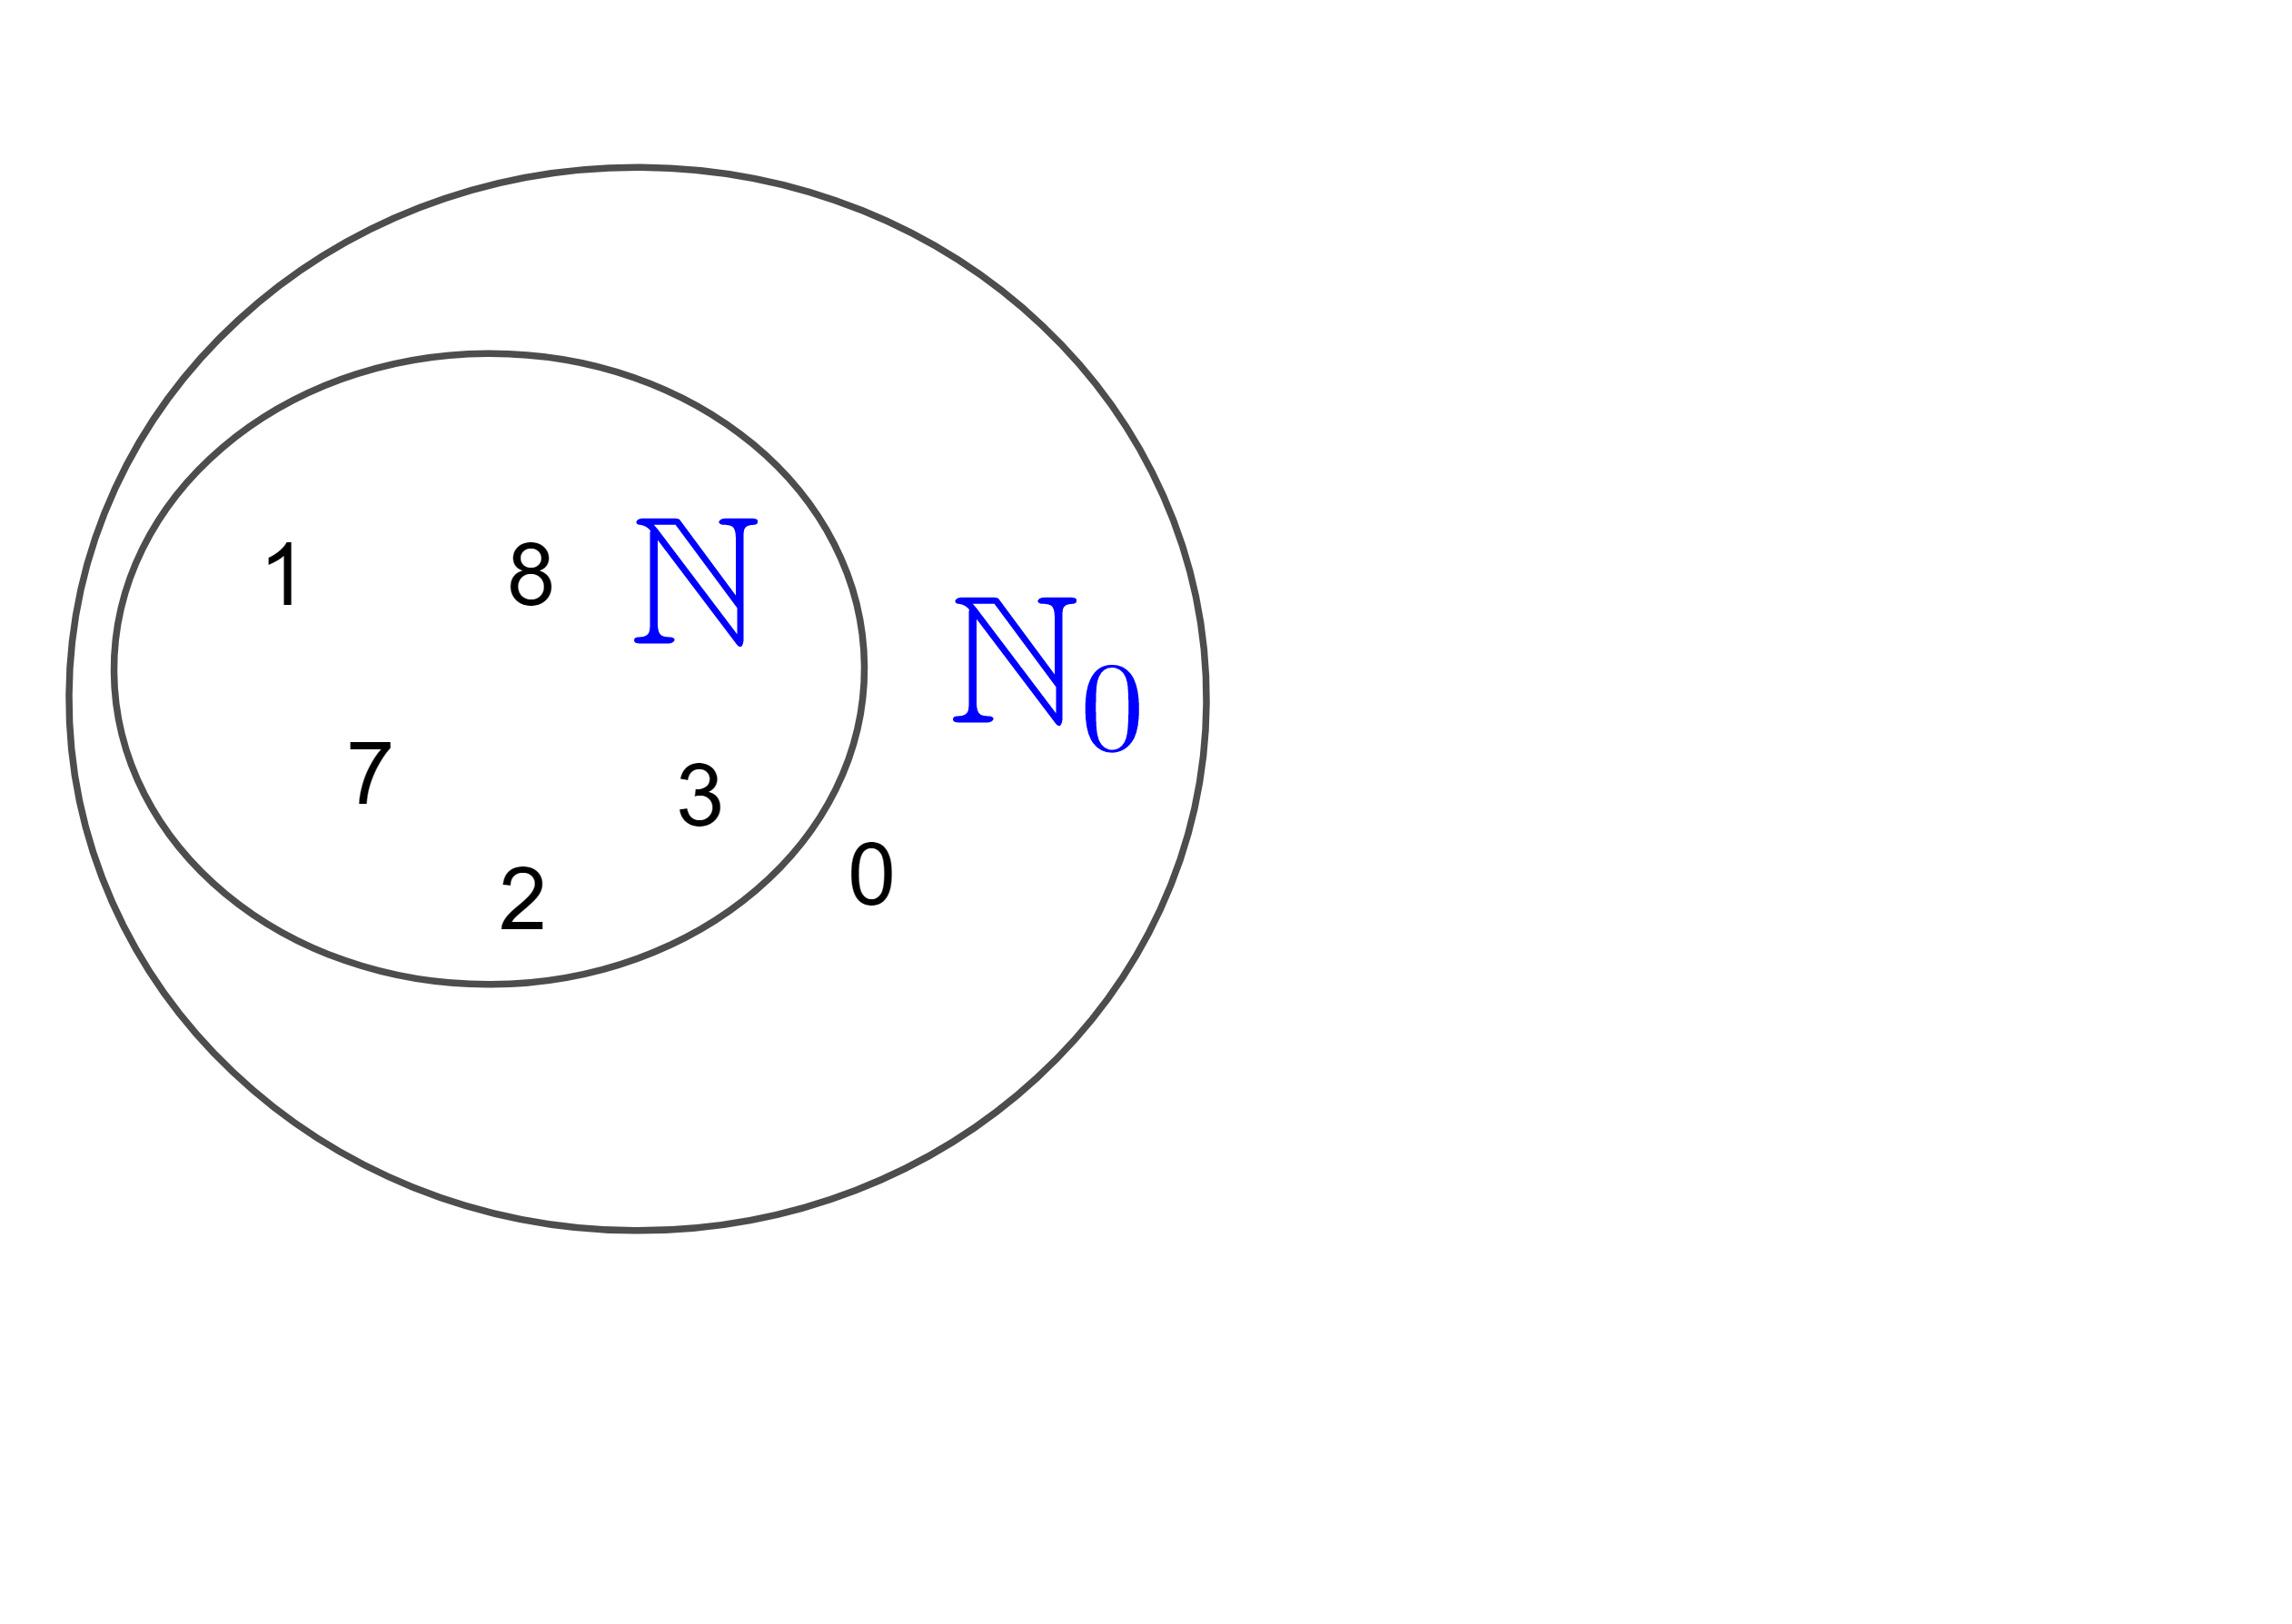
\includegraphics[width=\linewidth]{Image2.png}
\end{center}
\end{frame}

\begin{frame}
\frametitle{Los Numeros Enteros:}
\begin{center}
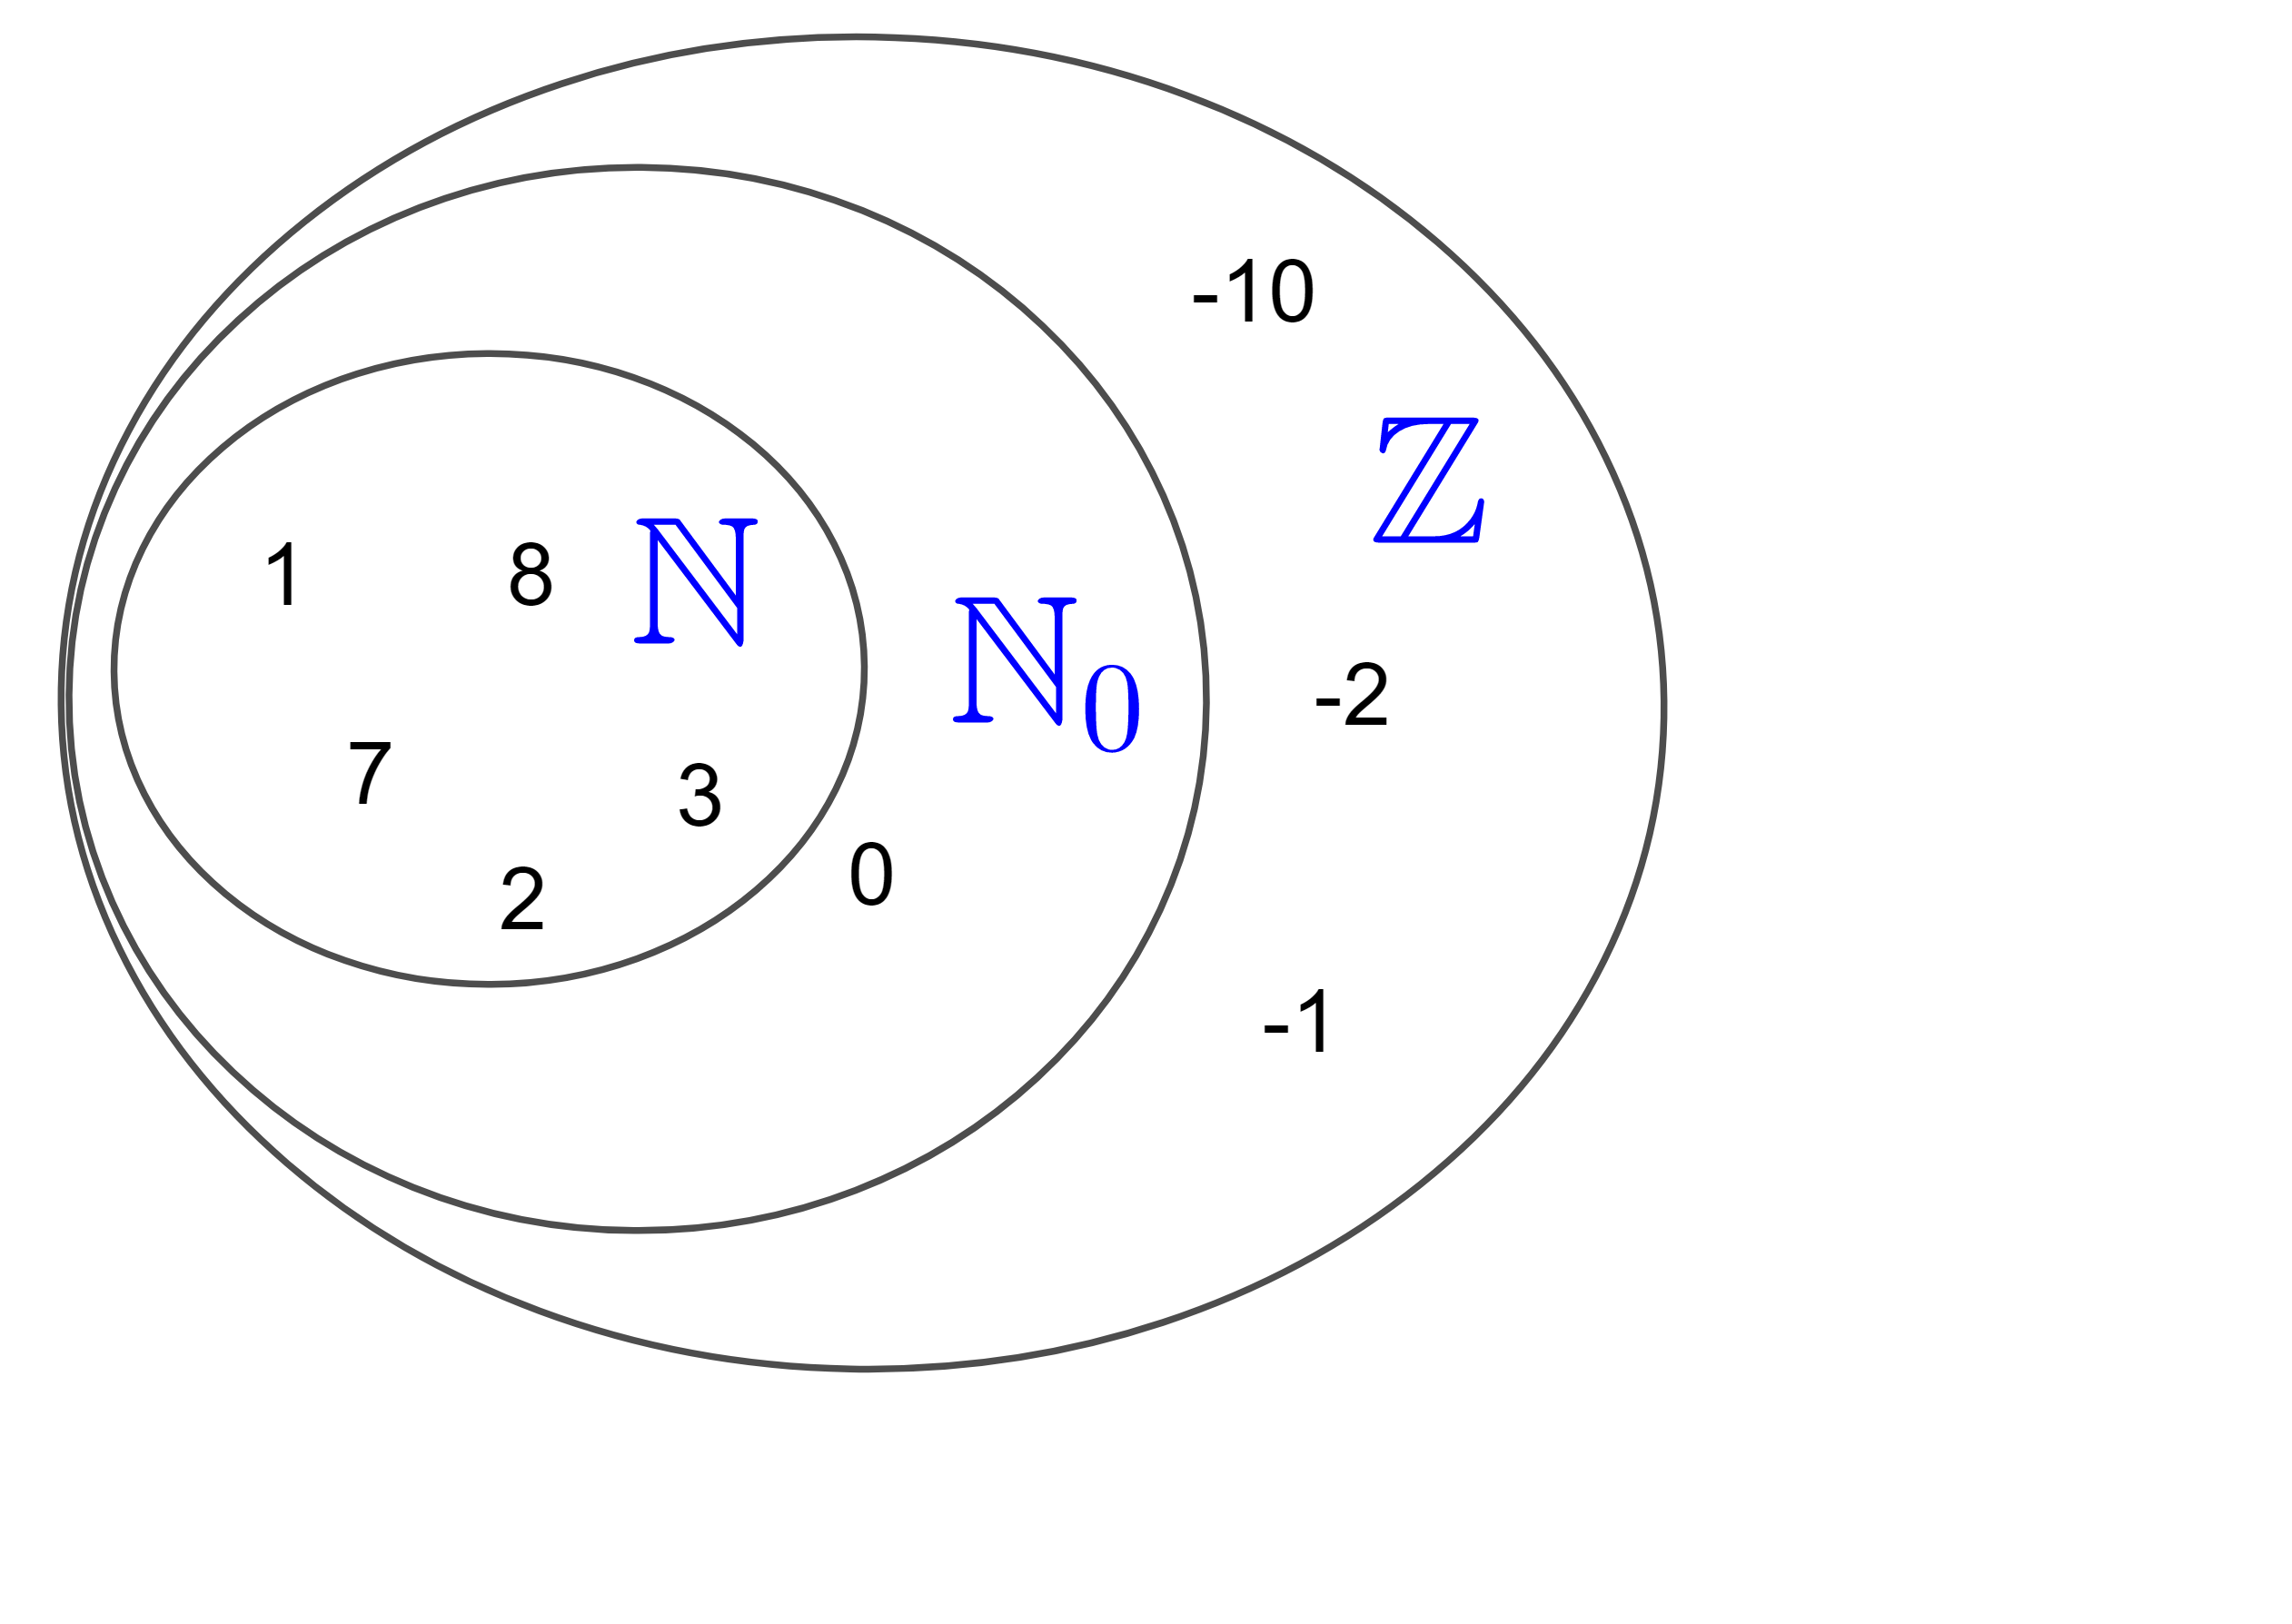
\includegraphics[width=\linewidth]{Image3.png}
\end{center}
\end{frame}


\begin{frame}
\frametitle{Los Numeros Enteros:}
Los numeros enteros fueron  muy utiles por muchisimo tiempo debido a que existen operaciones de suma, resta, multiplicacion y division.

$$3-1 =2 $$

$$2-5=-3 $$

$$\frac{4}{2}=2 $$

$$\frac{6}{2}=3 $$
\end{frame}

\begin{frame}
\frametitle{Los Numeros Enteros:}
{\huge{
Primer problema: }}
\vspace{10mm}
\begin{itemize}


\Large{
\item Cual es el significado de $\frac{5}{2}$ o $\frac{1}{3}$ ?}
\end{itemize}

\end{frame}


\begin{frame}
\frametitle{Los Numeros Racionales:}
\begin{center}
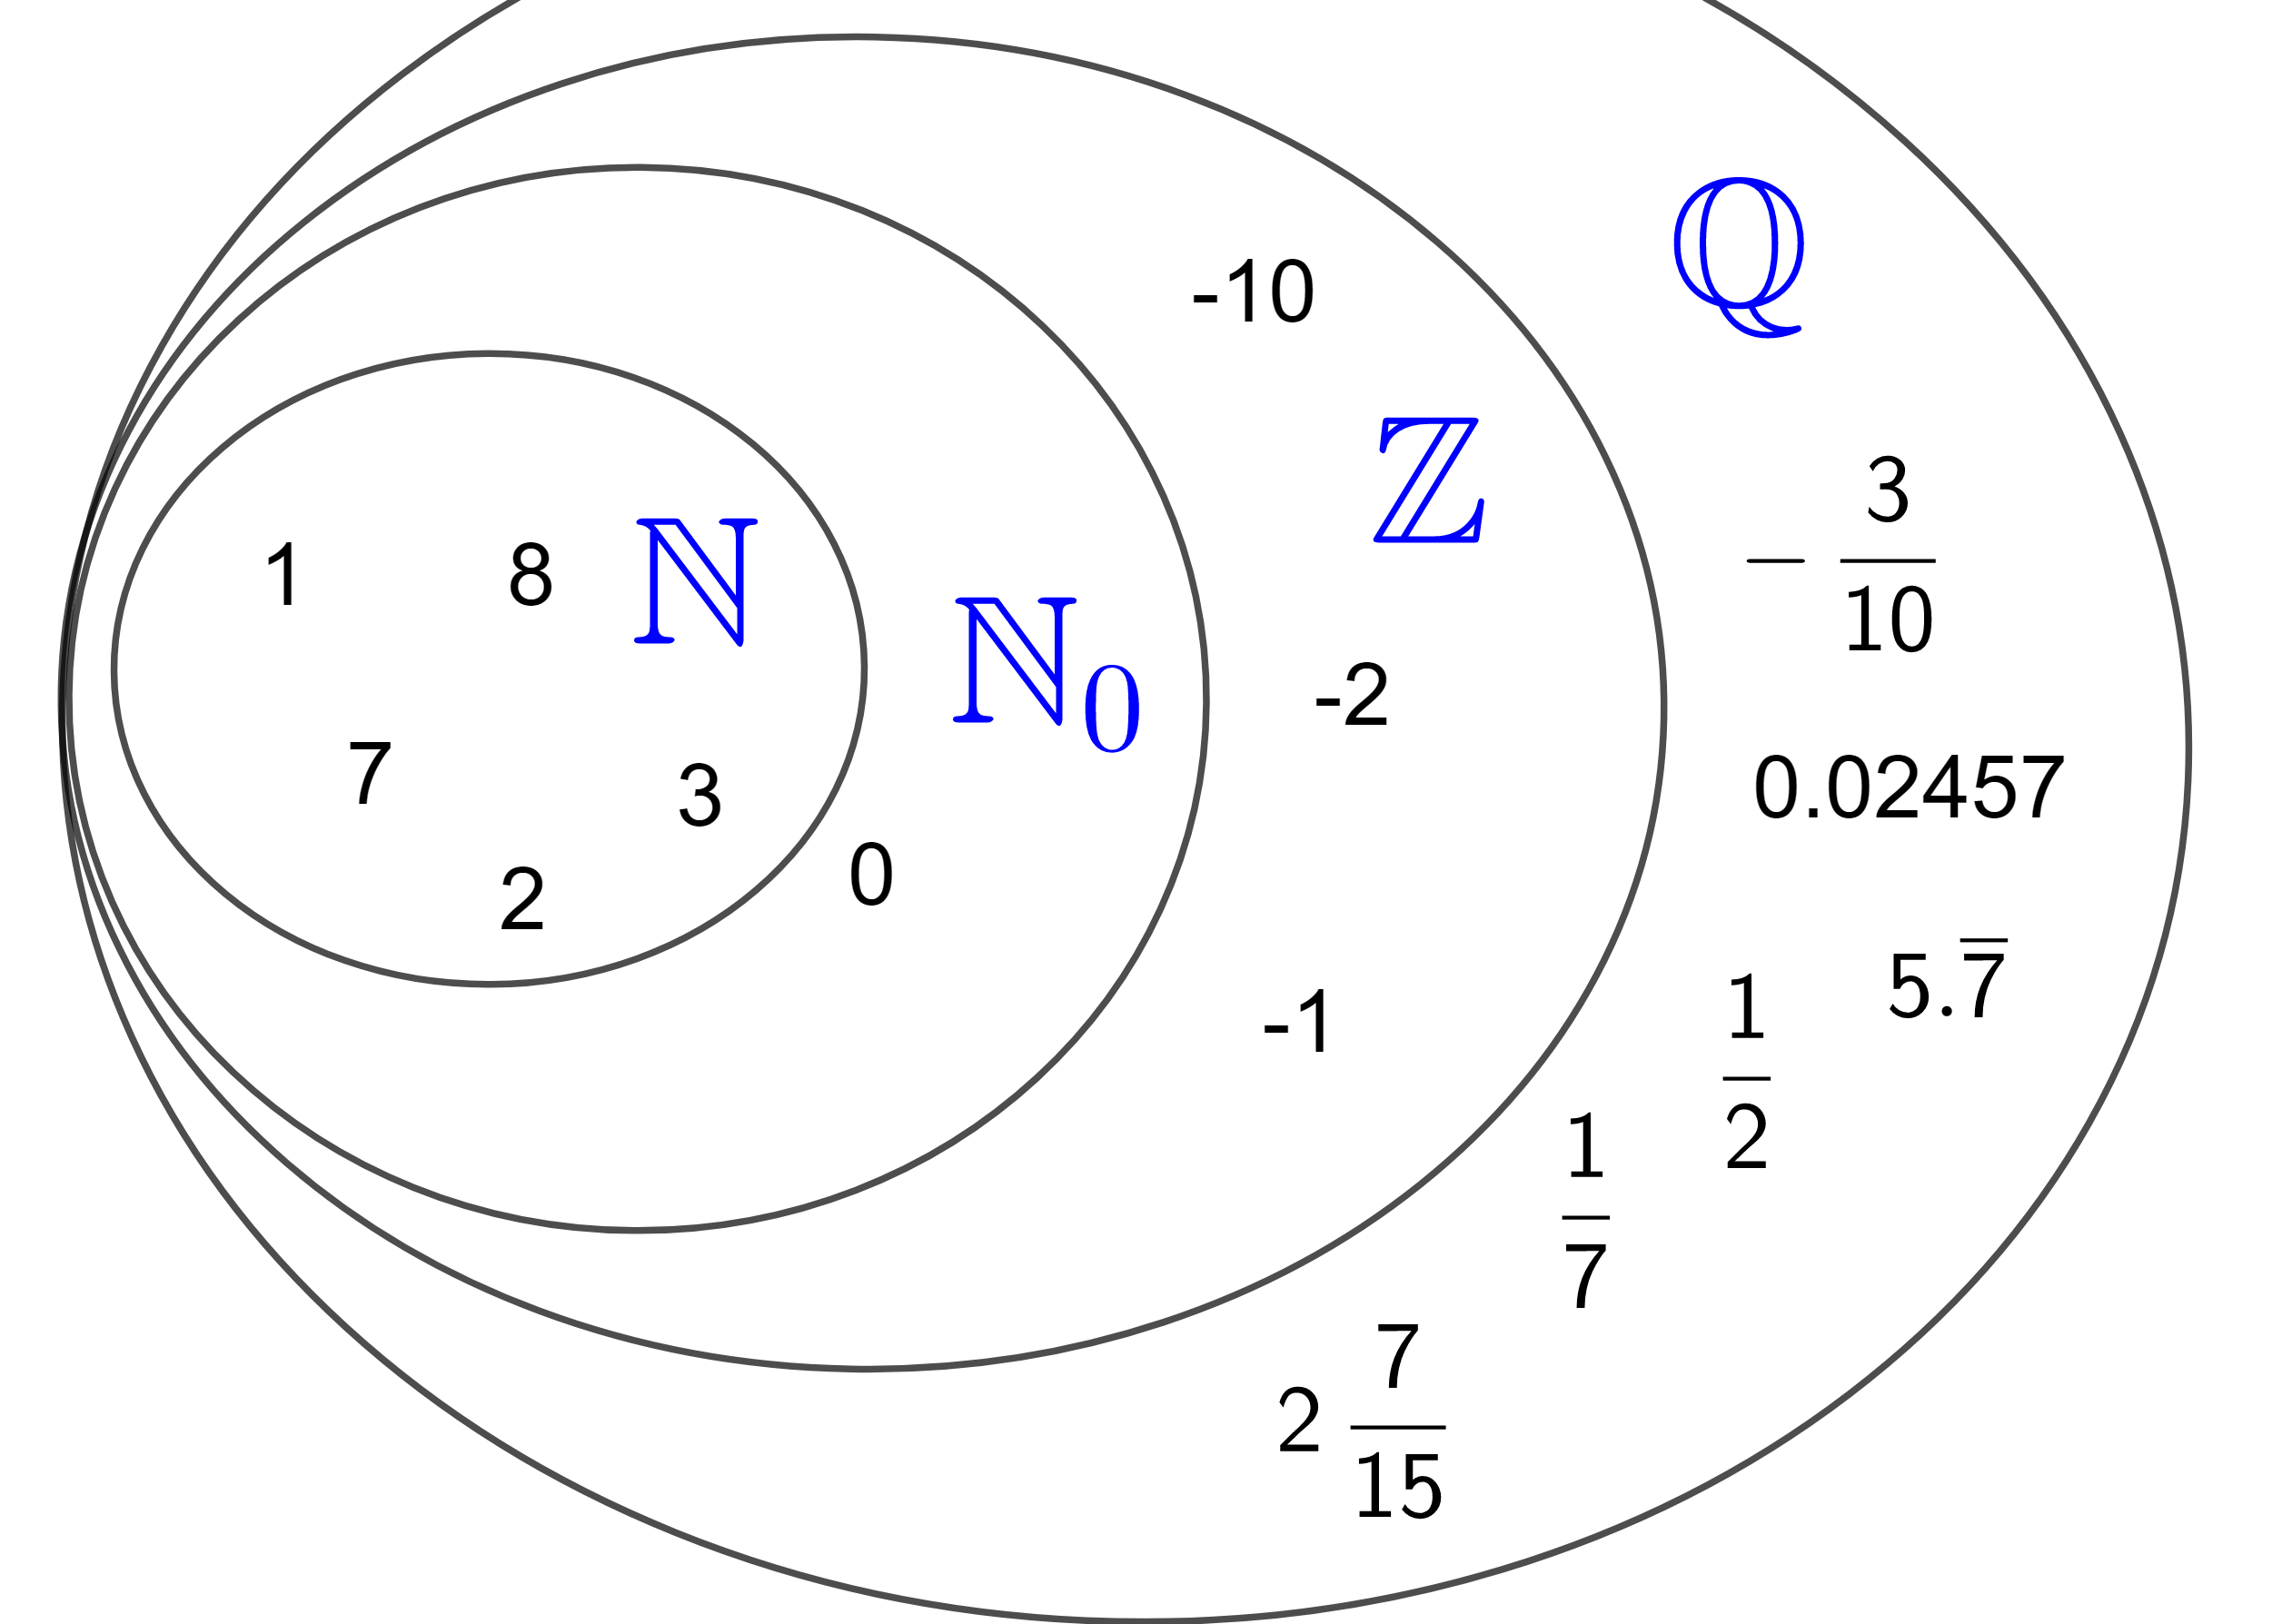
\includegraphics[width=0.75\linewidth]{Image4.png}
\end{center}
\end{frame}

\begin{frame}
\frametitle{Los Numeros Racionales:}
El mundo fue feliz por MUCHO TIEMPO con los numeros racionales.

\pause
\vspace{10mm}
Hasta que alguien descubriera que $\sqrt{2}$ no era un numero racionales.

\begin{itemize}
\item Leyenda

\item Recomiendo el libro: The square root of 2, David Flannery.
\end{itemize}
\end{frame}

\begin{frame}
\frametitle{Los Numeros Irracionales:}
\begin{center}
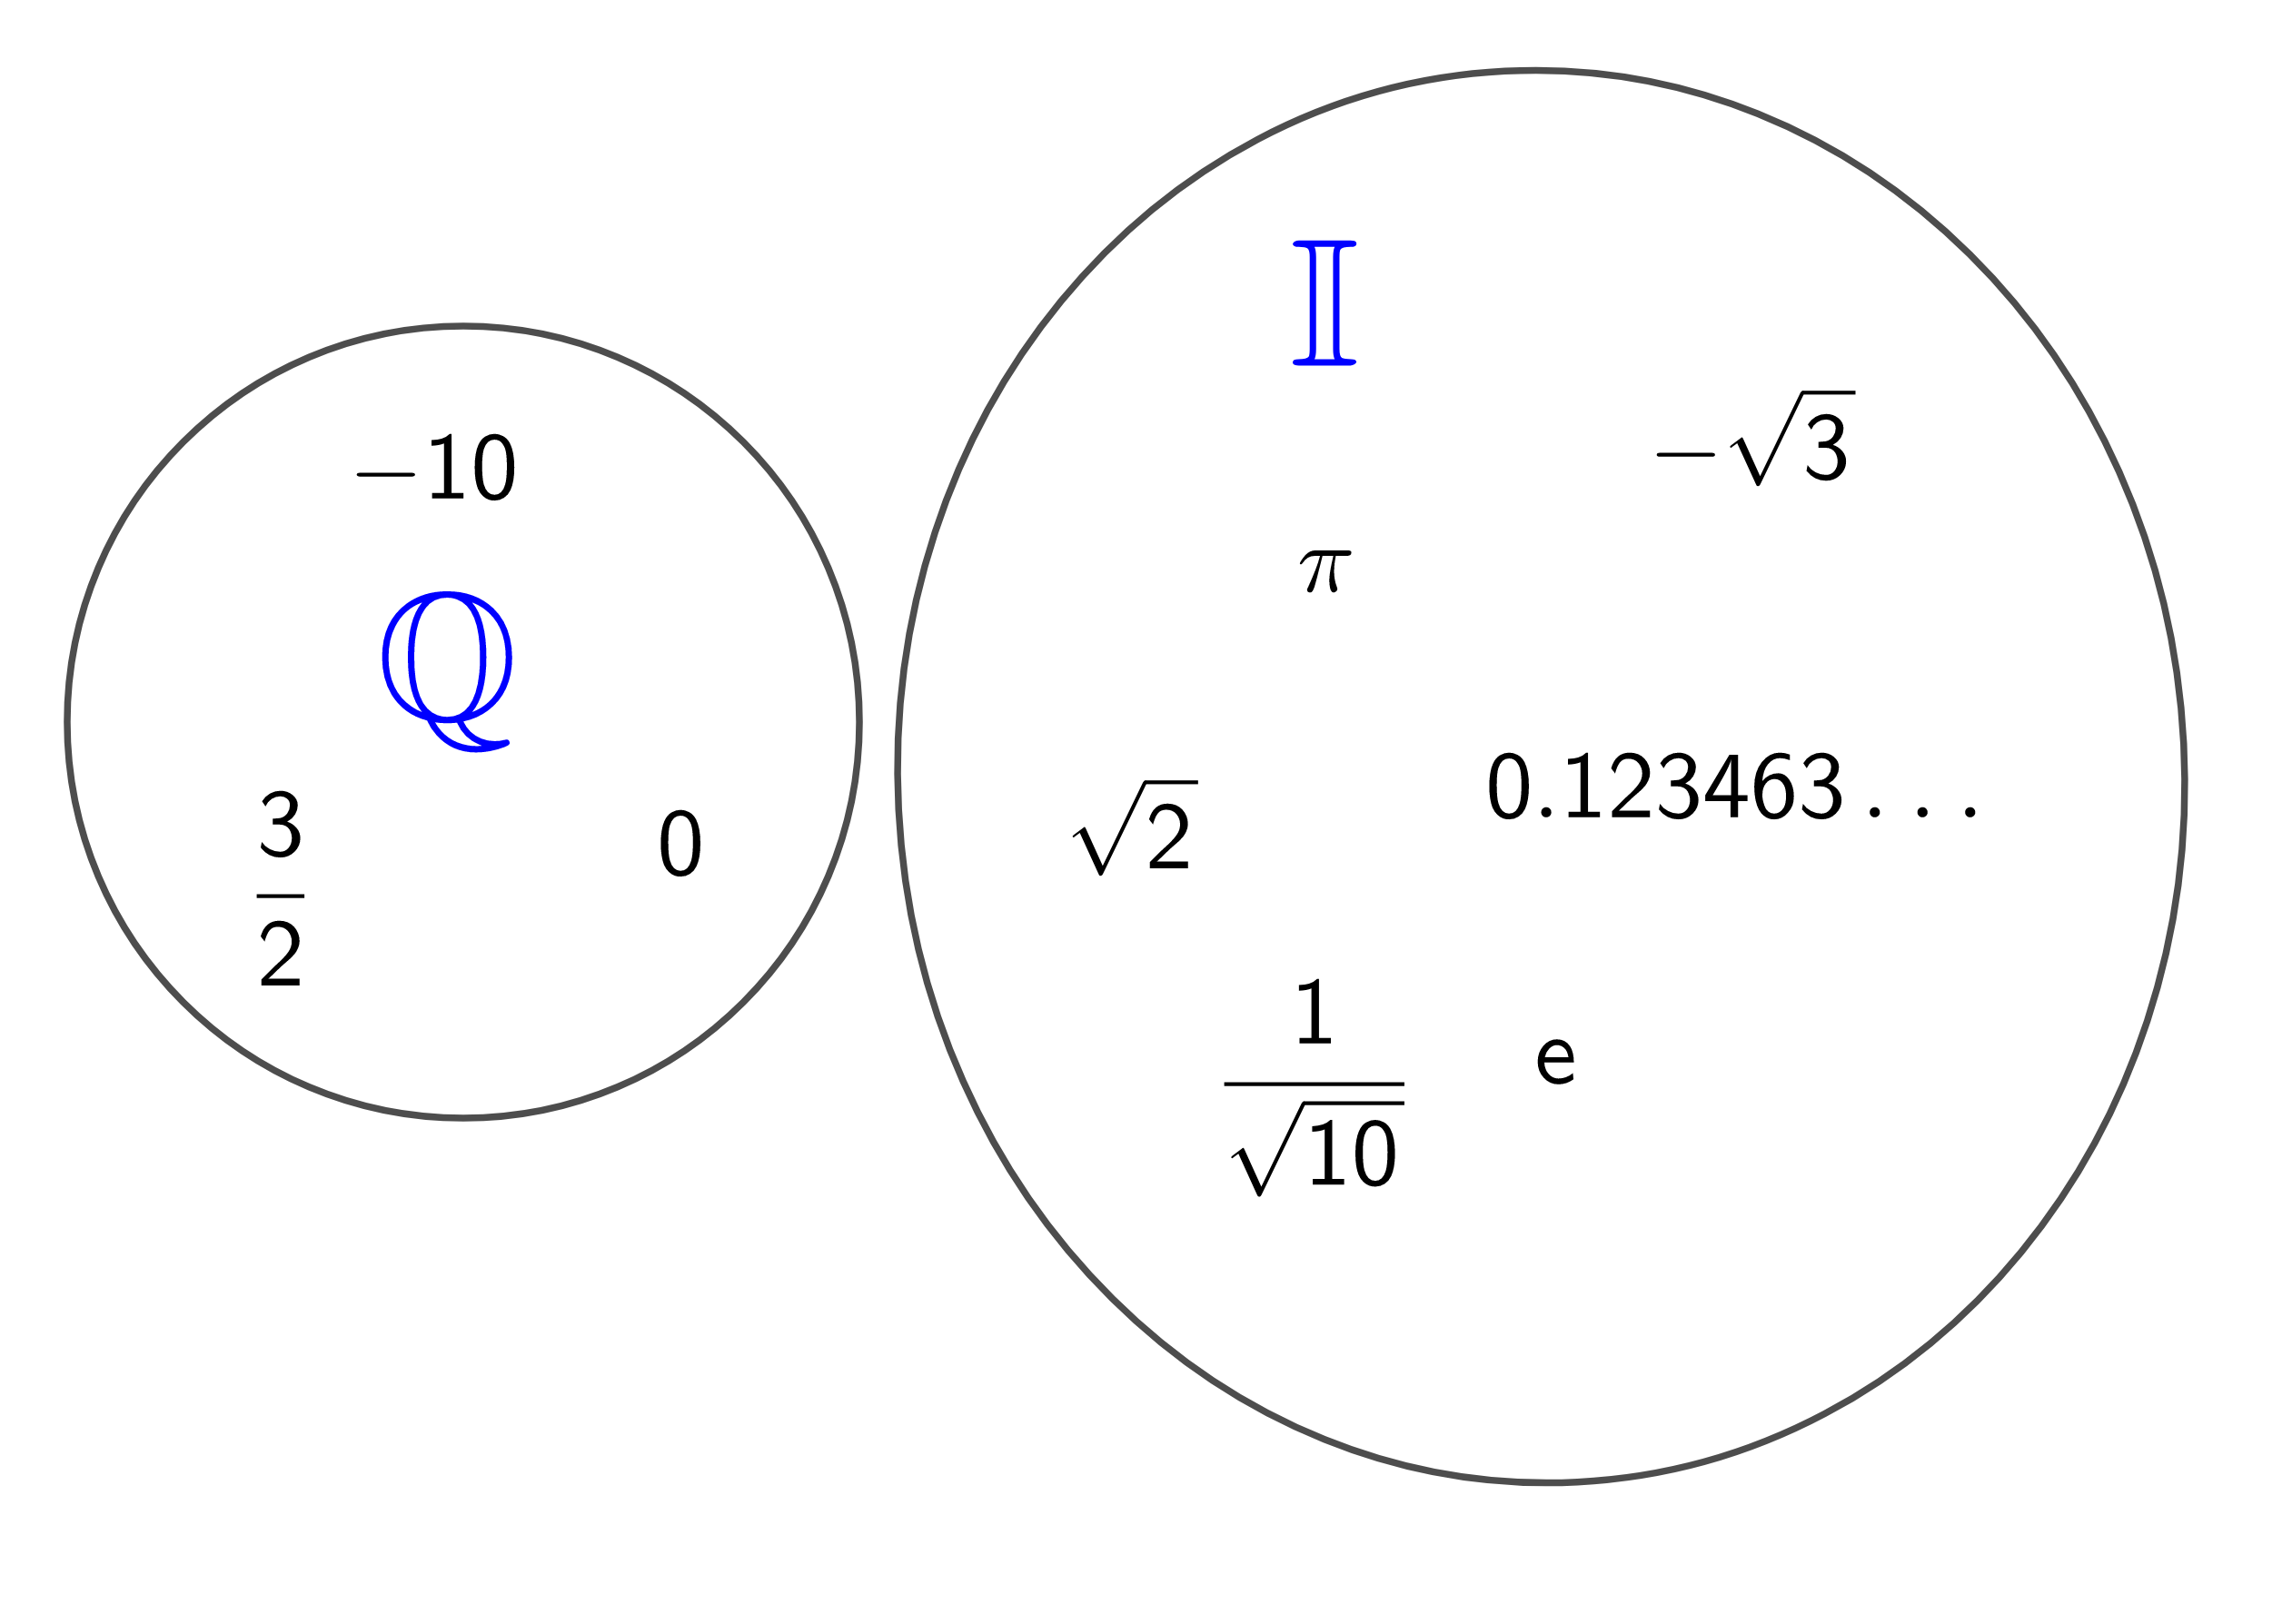
\includegraphics[width=0.8\linewidth]{Image5.png}
\end{center}
\end{frame}

\begin{frame}
\frametitle{Los Numeros Reales:}
\begin{center}
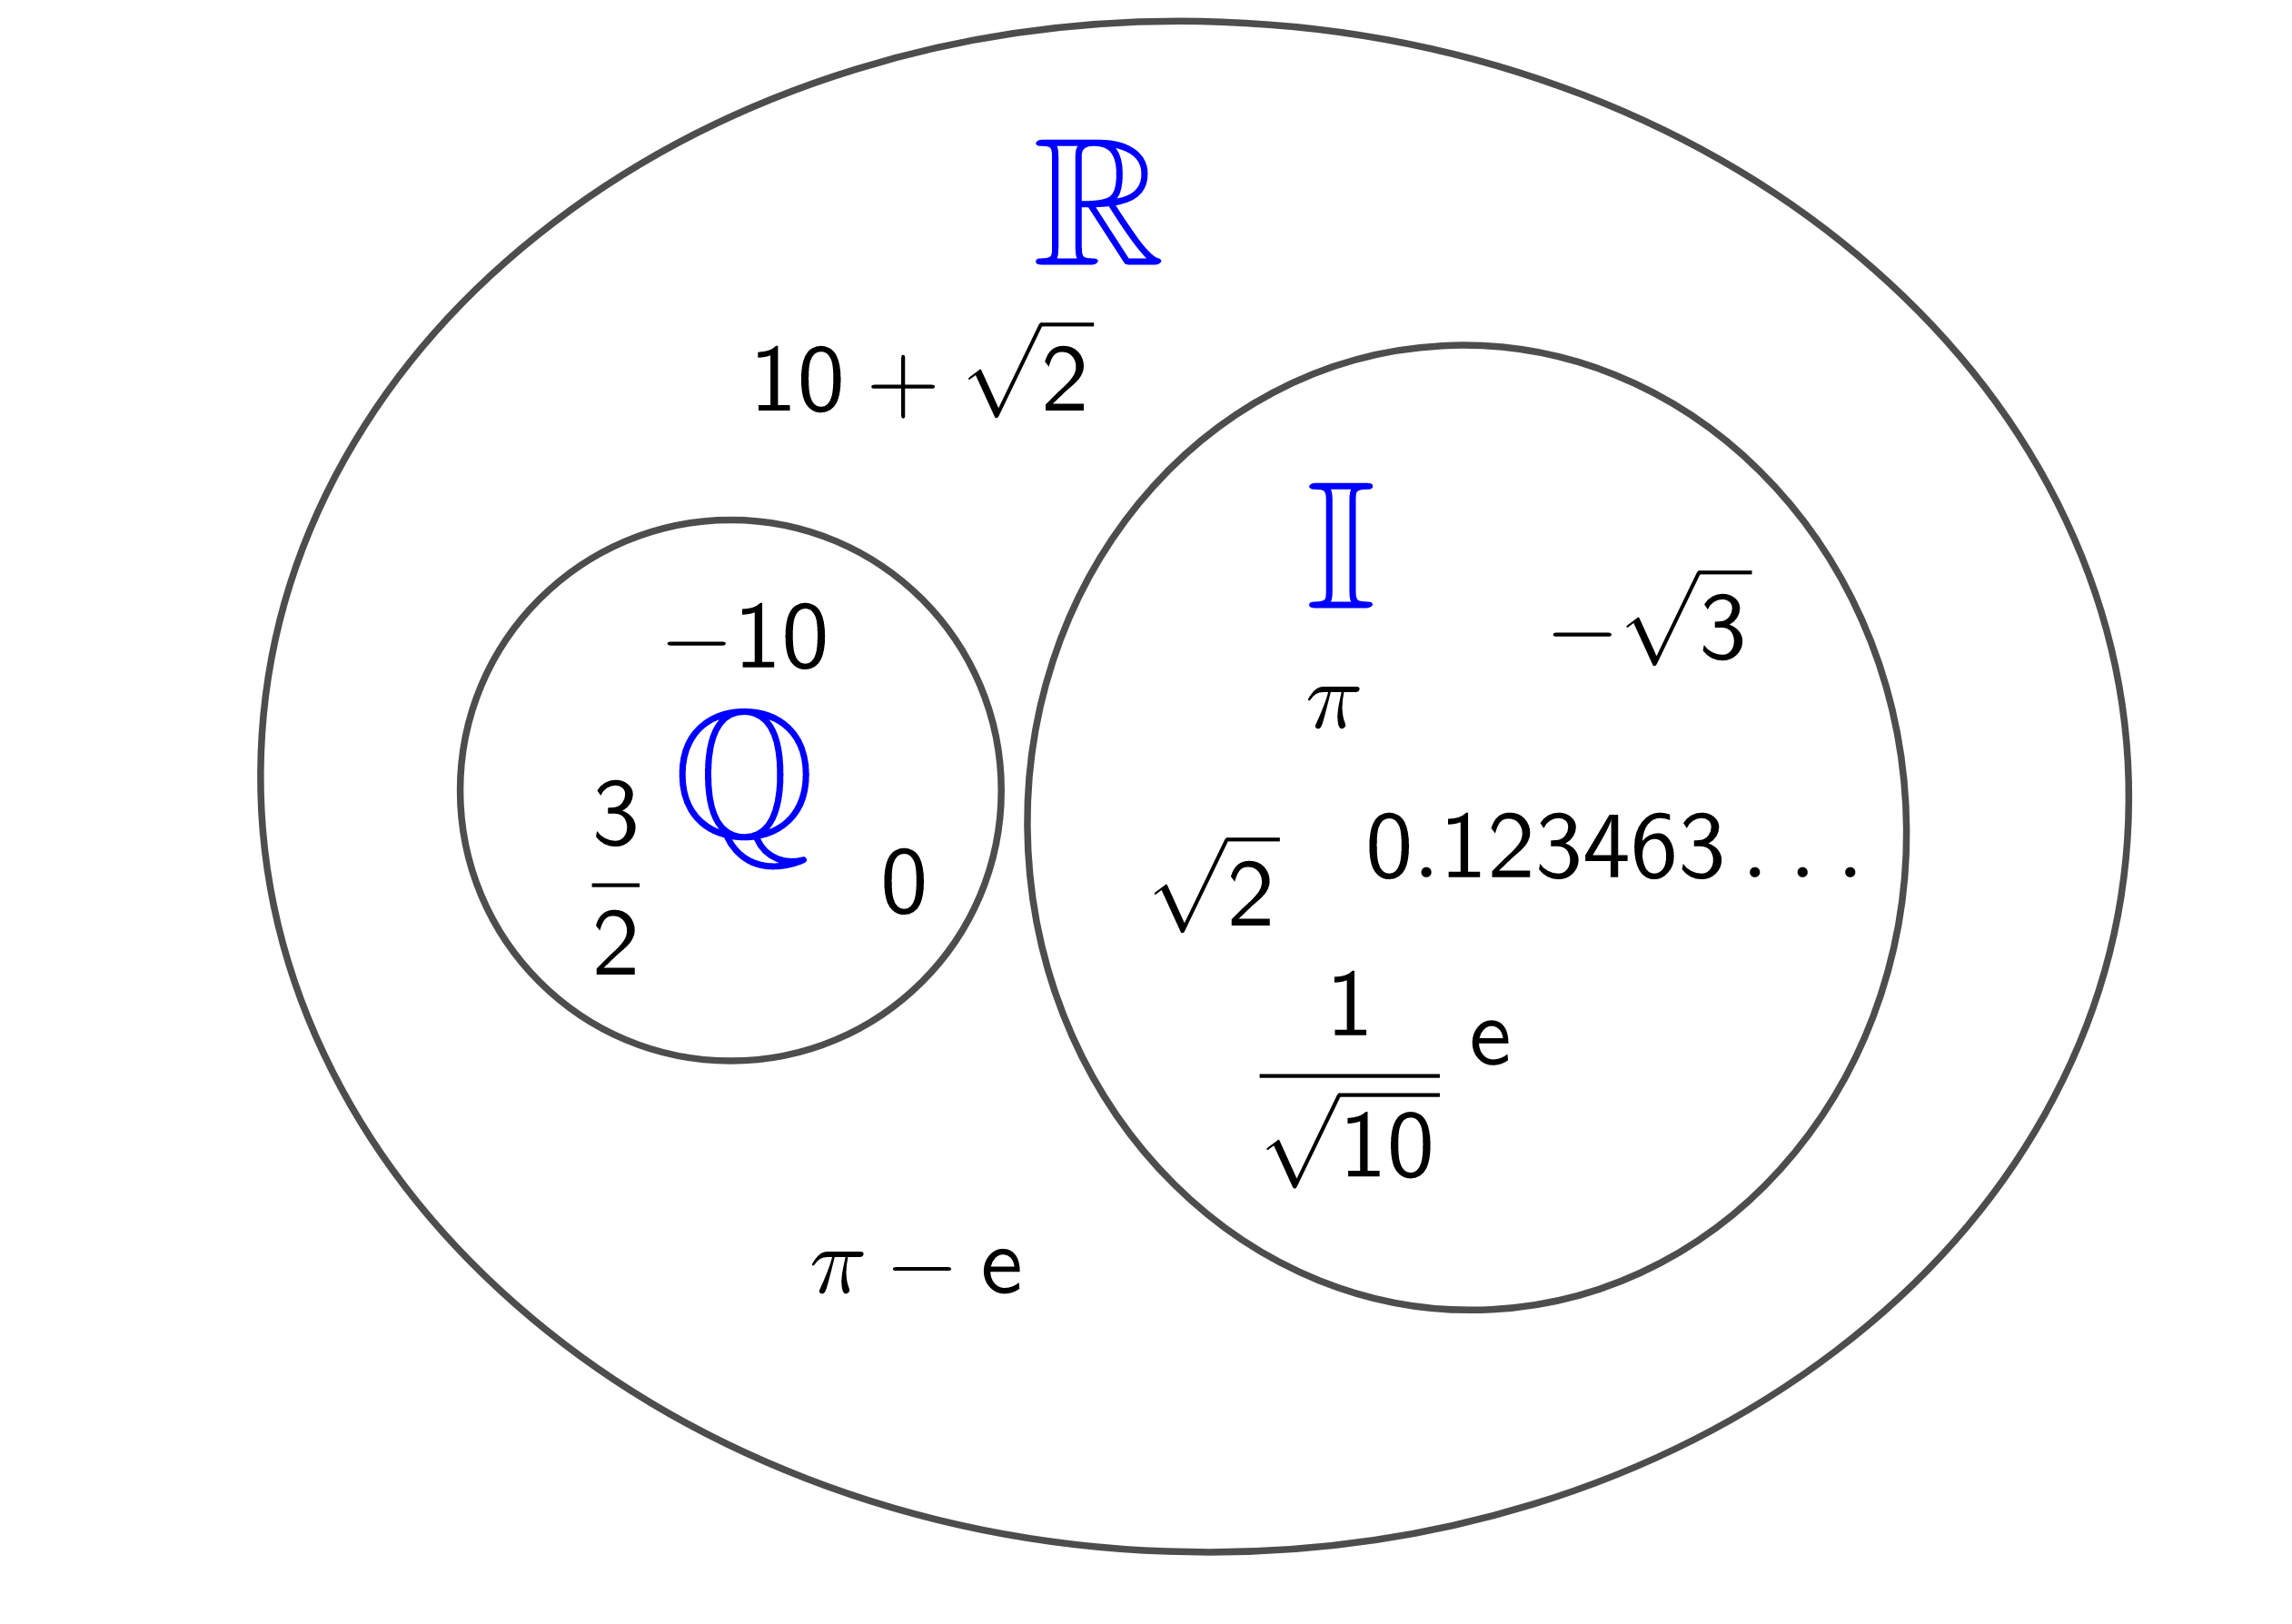
\includegraphics[width=0.8\linewidth]{Image6.png}
\end{center}
\end{frame}

\begin{frame}
\frametitle{Los Numeros Reales:}
{\huge{
Segundo problema: }}
\vspace{10mm}
\begin{itemize}


\Large{
\item Podemos resolver la ecuacion $x^2=-1?$}
\end{itemize}

\pause
\vspace{5mm}
Podemos tomar la raiz cuadrada y tenemos que $x=\pm\sqrt{-1}$.

\end{frame}

\begin{frame}
\frametitle{Los Numeros Complejos:}
Con esta motivacion Rafael Bombell en 1526 invento los numeros complejos. 

\pause
\vspace{5mm}
Su idea fue formalizar el concepto de $\sqrt{-1}$ la que llamo unidad compleja.

\pause
\vspace{5mm}
\begin{itemize}
\item $i=\sqrt{-1}$ 


\item Les recomiendo el libro: An imaginary tale of the story of $\sqrt{-1}$, Paul Nahin.
\end{itemize}
\end{frame}

\begin{frame}
\frametitle{Los Numeros Complejos:}
\begin{center}
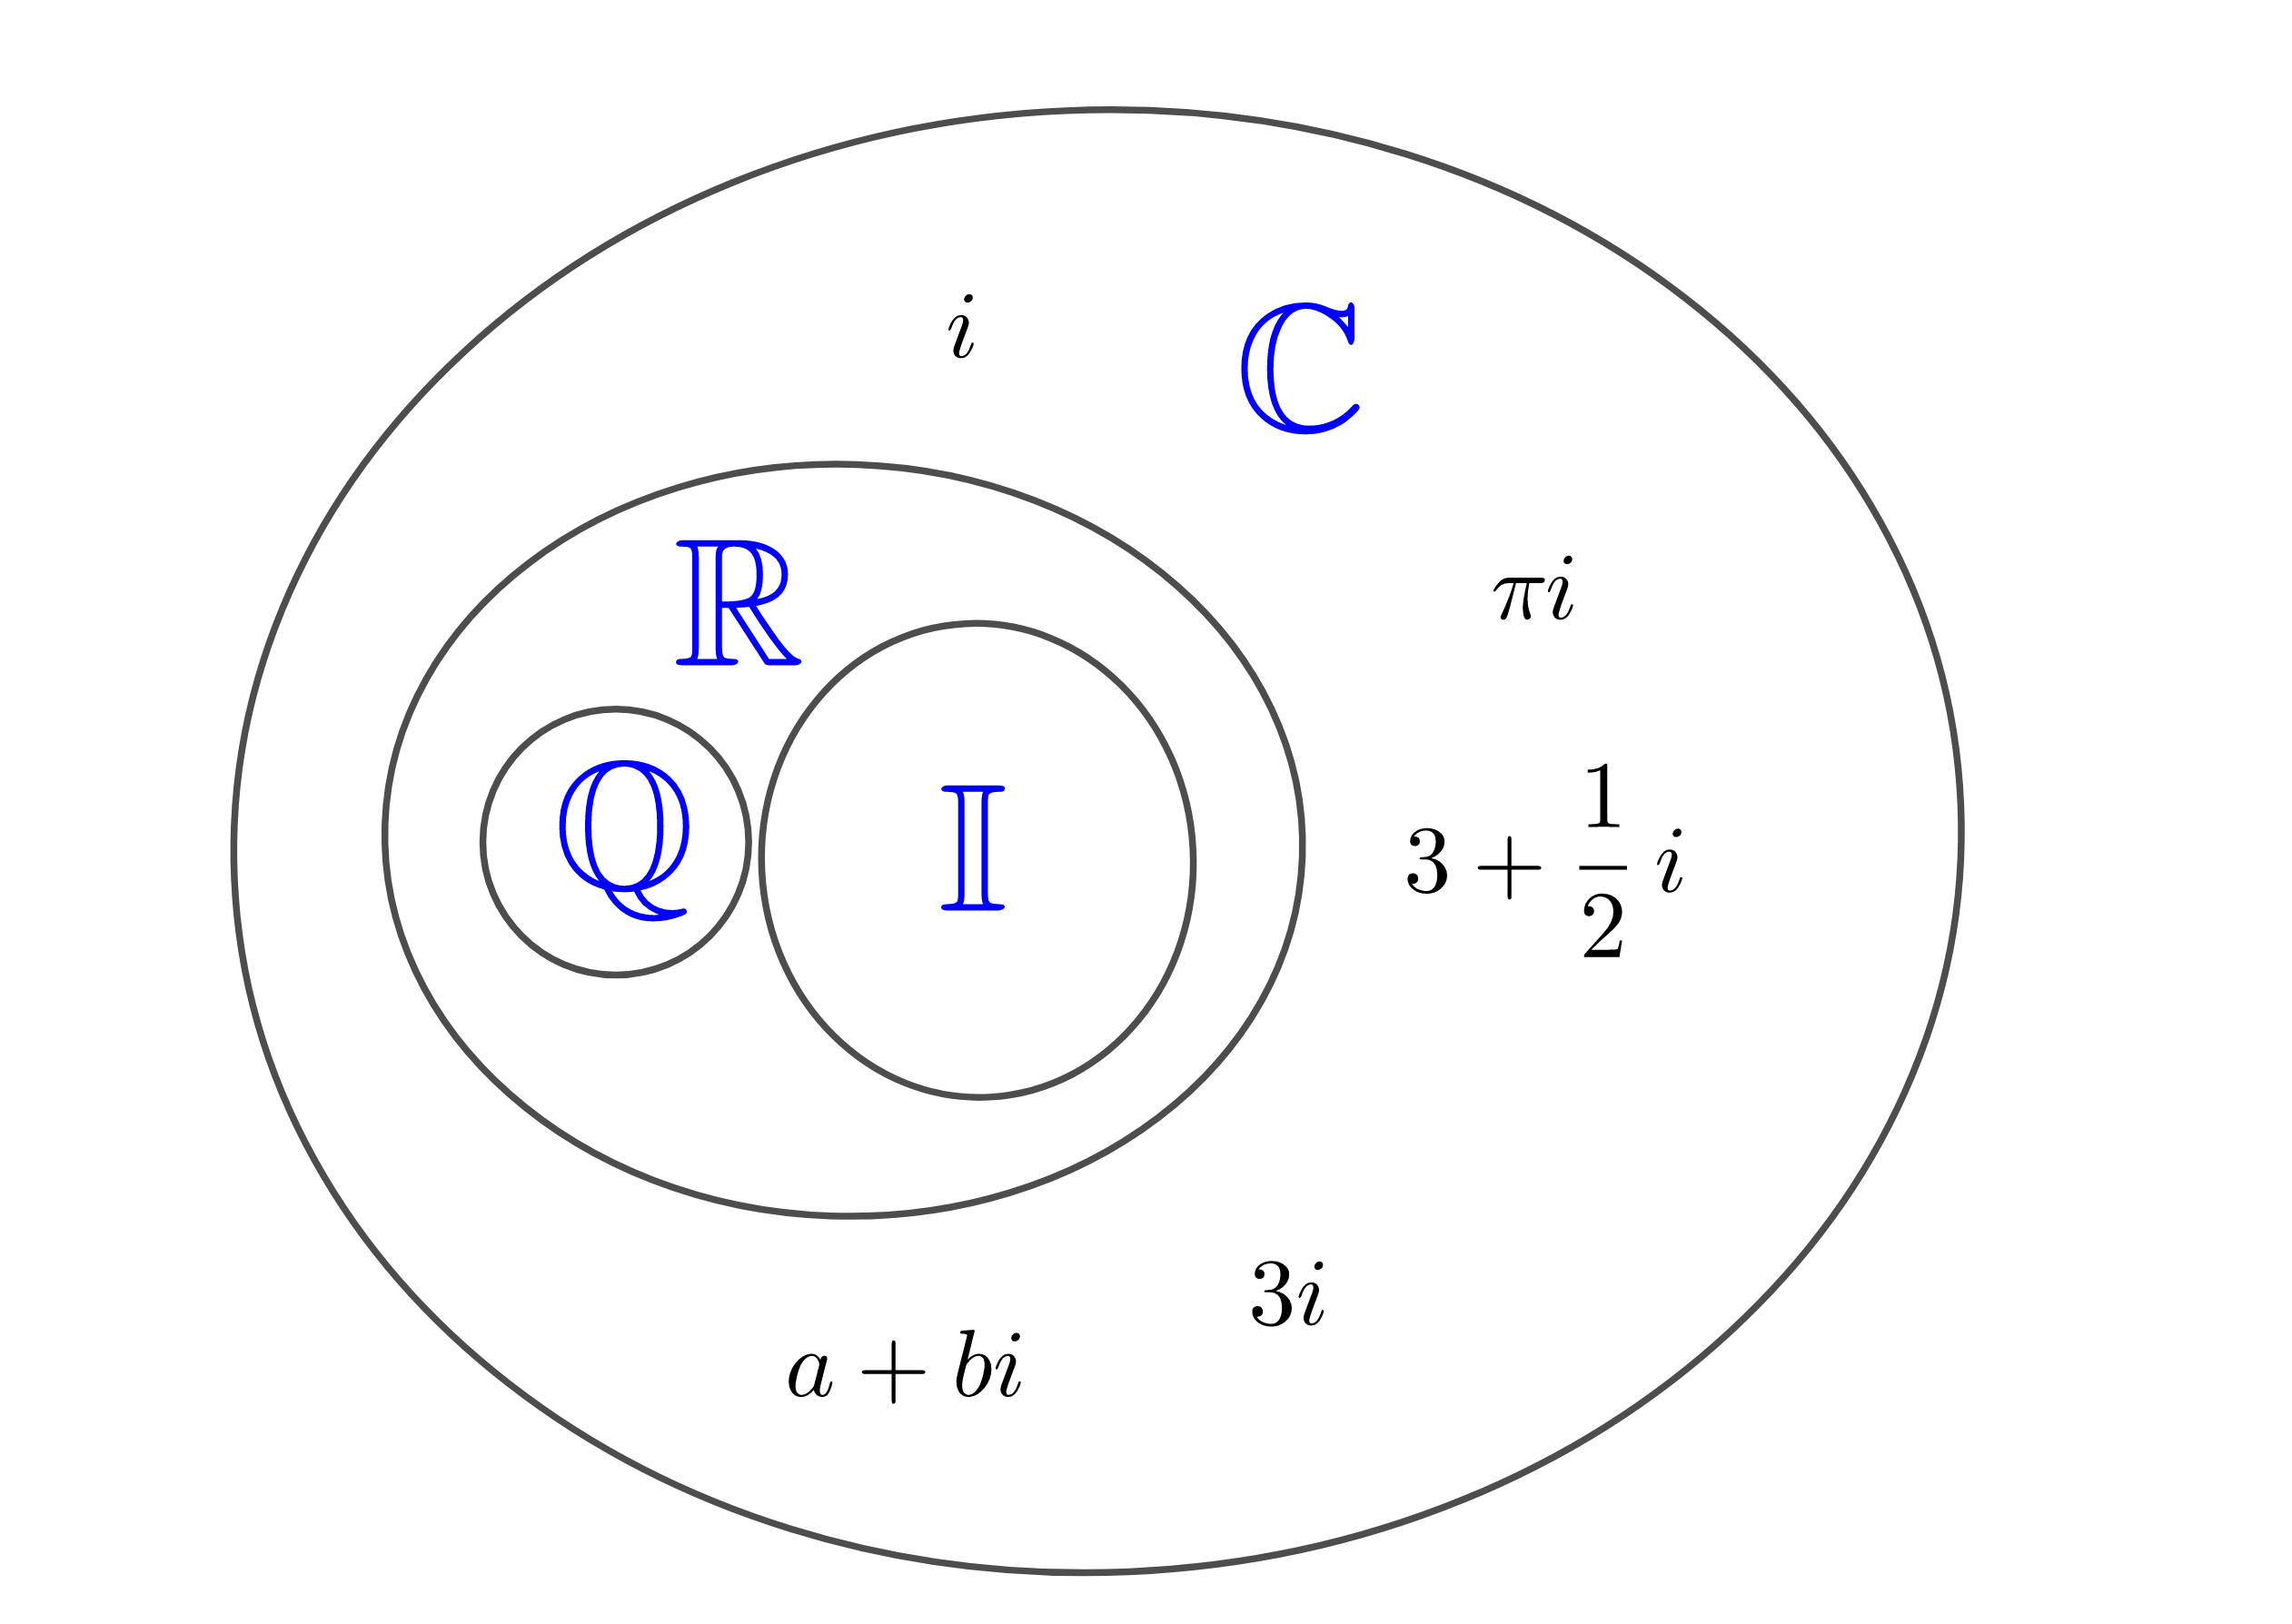
\includegraphics[width=0.8\linewidth]{Image7.png}
\end{center}
\end{frame}


\begin{frame}
\frametitle{Resumen:}

\begin{enumerate}
\item PARTE I: Sistemas de Numericos
\begin{itemize}
\item $\NN$
\item $\QQ$
\item $\RR$
\item $\CC$
\end{itemize}

\item PARTE II: Numeros Gaussianos
\begin{itemize}
\item Operaciones $+$ y $*$
\item Primos Gaussianos
\end{itemize}


\item PARTE III: 
\begin{itemize}
\item Sobre mi

\item Preguntas
\end{itemize}
\end{enumerate}
\end{frame}


\begin{frame}
\frametitle{Generalizando los numeros enteros}

Nos gustan los numeros enteros $\mathbb{Z}$ porque son numeros interesante, podemos sumar, restar y multiplicar.

\pause
Ademas, son utiles para contar y tienen bloques contructores llamados primos.


\vspace{5mm}

$$10=5\cdot 2 $$
$$7=7 $$
$$10=5\cdot 2 $$
$$15=5\cdot 3 $$
$$-12=-2\cdot 2 \cdot 3 $$
$$28=2\cdot 2 \cdot 7 $$
\end{frame}

\begin{frame}
\frametitle{Los numeros gaussianos}
Primero generalizamos el conjunto en el que queremos trabajar.

\begin{center}
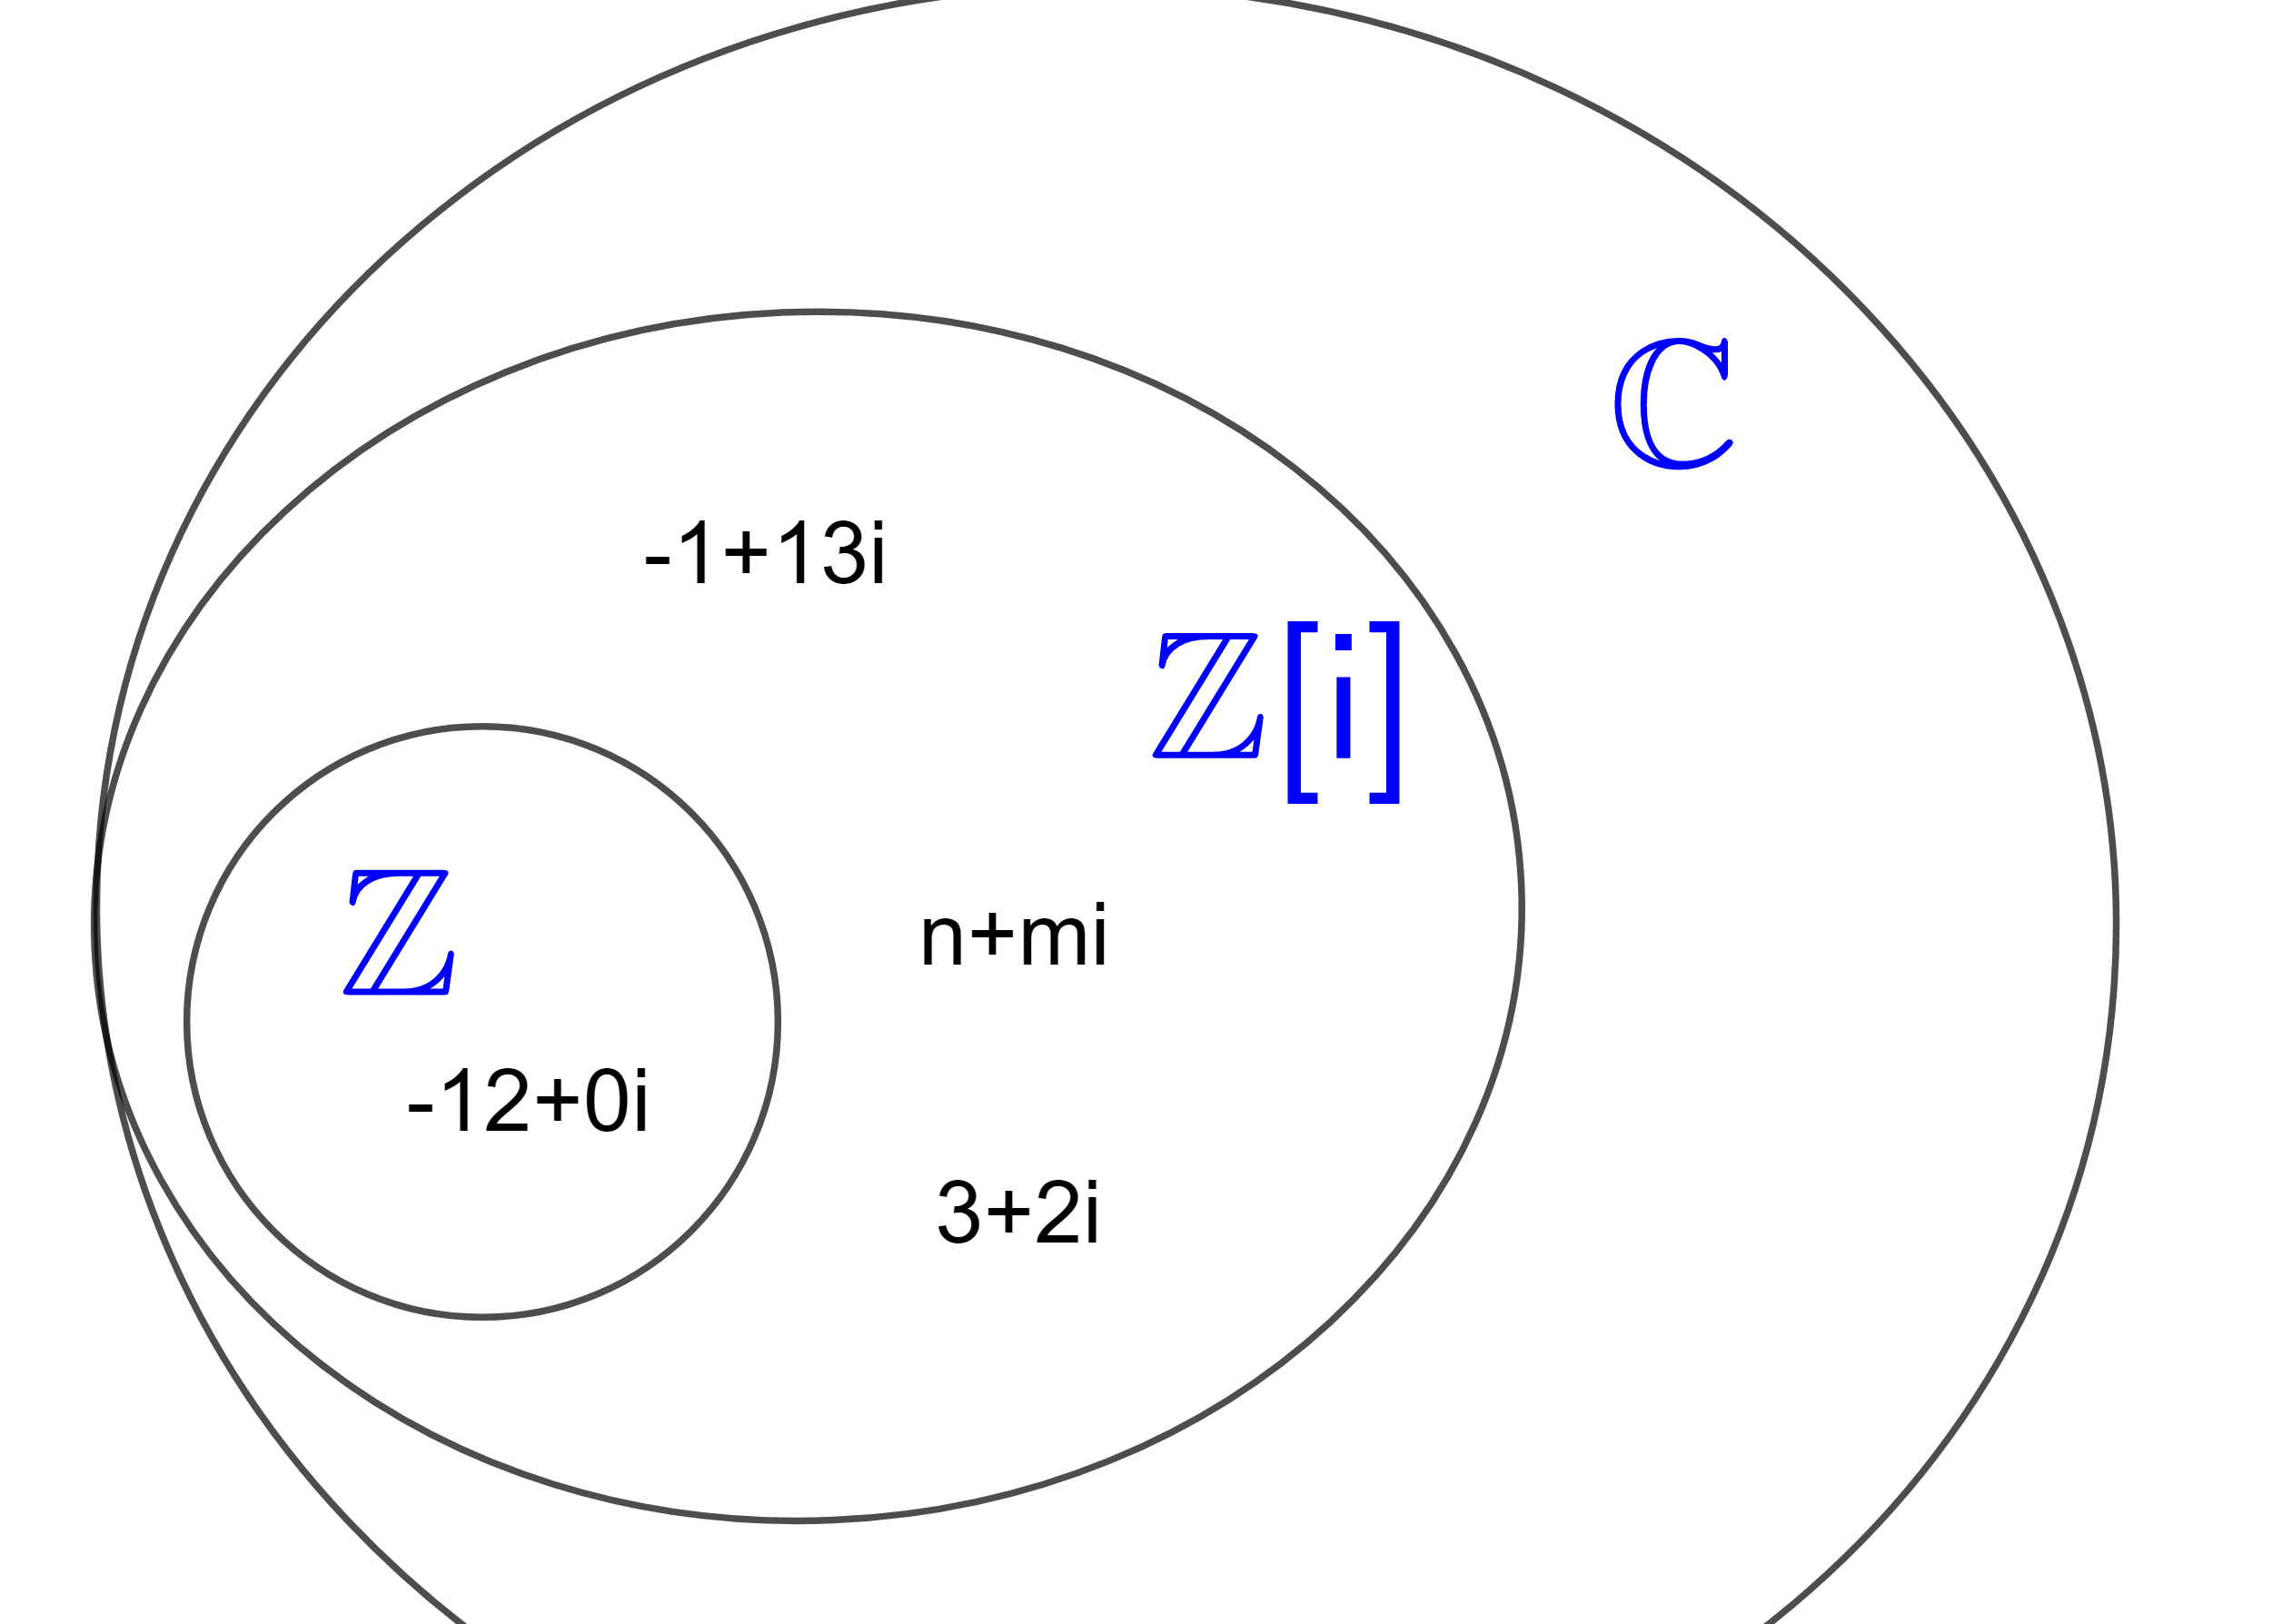
\includegraphics[width=0.8\linewidth]{Image8.png}
\end{center}

\end{frame}


\begin{frame}
\frametitle{Operaciones en los numeros gaussianos}
Ahora que tenemos nuestro conjunto nos gustaria Sumar, Restar y Multiplicar numeros gaussianos.

$$2-5i+5+2i=7-3i $$
\pause
$$1+i-3i=1-2i $$

\pause
$$(1-3i)*(1+3i)=-8 $$

\pause
$$(i)*(2-5i)=2i-5i^2=5+2i $$

\end{frame}

\begin{frame}
\frametitle{Primos}
Podremos hablar sobre primos en los enteros gaussianos? 

\pause
\vspace{10mm}
 Es decir, son los numeros primos (que nosotros conocemos) bloques fundamentales para todos los numeros gaussianos?

\pause
\vspace{10mm}
Si podemos hablar sobre bloques contructores ALIAS primos. 

\pause PERO no son los mismos primos.
\end{frame}

\begin{frame}
\frametitle{Primos}
Estudiemos los numeros primos e intentemos deducir cuales son los bloques contructores. A los que empezare a llamar primos gaussianos.
$$2\pause =(1+i)(1-i) $$
\pause
$$3\pause =3=(a+bi)(c+di) $$
\pause
$$5\pause =(2+i)(2-i) $$
\pause
$$7\pause =7=(a+bi)(c+di) $$
\pause
$$11\pause =11=(a+bi)(c+di) $$
\pause
$$13\pause =(3+2i)(3-2i) $$
\end{frame}




\begin{frame}
\frametitle{Primos Gaussianos}
Classifiquemos TODOS los primos (en el sentido classico) $2, 3, 5, 7, 11, 13, 17, 19, 23,\ldots$ en tres grupos.

\pause
El primer grupo es uno bien especial es el
$$\{2\}$$

\pause
El segundo grupo son los primos que cuando son divididos por 4 dejan un resto de 3.
$$\{3,7,11,19,23,\ldots\}$$

\pause
El tercer grupo son los primos que cuando son divididos por 4 dejan un resto de 1.
$$\{5,7,11,19,23,\ldots\}$$
\end{frame}


\begin{frame}
\frametitle{Teorema para el primer grupo}
\begin{theorem}
El 2 da nacida a dos primos gaussianos que son $1+i$ y $1-i$.
\end{theorem}

\end{frame}

\begin{frame}
\frametitle{Teorema para el segundo grupo}
\begin{theorem}
Los primos que cuando son divididos por 4 dejan un resto de 3.
$$\{3,7,11,19,23,\ldots\}$$
Todos los numeros primos en este grupo son efectivamente \textbf{primos gaussianos}.
\end{theorem}
\end{frame}

\begin{frame}
\frametitle{Teorema para el tercer grupo}
\begin{theorem}
Los primos que cuando son divididos por 4 dejan un resto de 1.
$$\{5,7,11,19,23,\ldots\}$$
Todos los numeros primos en este grupo \textbf{NO SON} numeros gaussianos.

\pause 
De hecho, cada uno de ellos engendra dos numeros gaussianos que no estaban en los enteros. 

Ellos son de la forma $a+bi$ con $a^2+b^2=p^2$ y $p$ un primo en este conjunto.
\end{theorem}


\end{frame}

\begin{frame}
\frametitle{Un libro mas}

\Large{El ultimo libro que quiero recomendarles es muy reciente escrito por el presidente de la sociedad de matematicas chilena y professor de la USACH.

\vspace{10mm}
Un Viaje a las ideas, 33 historias matematicas asombrosas por Andres Navas}

\end{frame}


\begin{frame}
\frametitle{Resumen:}

\begin{enumerate}
\item PARTE I: Sistemas de Numericos
\begin{itemize}
\item $\NN$
\item $\QQ$
\item $\RR$
\item $\CC$
\end{itemize}

\item PARTE II: Numeros Gaussianos
\begin{itemize}
\item Operaciones $+$ y $*$
\item Primos Gaussianos
\end{itemize}


\item PARTE III: 
\begin{itemize}
\item Sobre mi

\item Preguntas
\end{itemize}
\end{enumerate}
\end{frame}

\end{document}

%\begin{mydef}
%A dynamical system is a pair $(S,\phi)$ consisting of a set $S$ and a self-map $\phi:S\to S$.
%\end{mydef}
